\documentclass[a4paper,12pt]{article}

\usepackage[margin=2cm]{geometry}
\usepackage{verbatim}% http://ctan.org/pkg/verbatim
\usepackage{xcolor}
\usepackage{graphicx}

\title{List of lists of references -- Follow the links: Solution}
\author{}
\date{}

\begin{document}

\maketitle

The typical student \textbf{expectation} of what code like this would do like is create a two dimensional array holding all numbers from 0 to 15 as below.
\bigskip

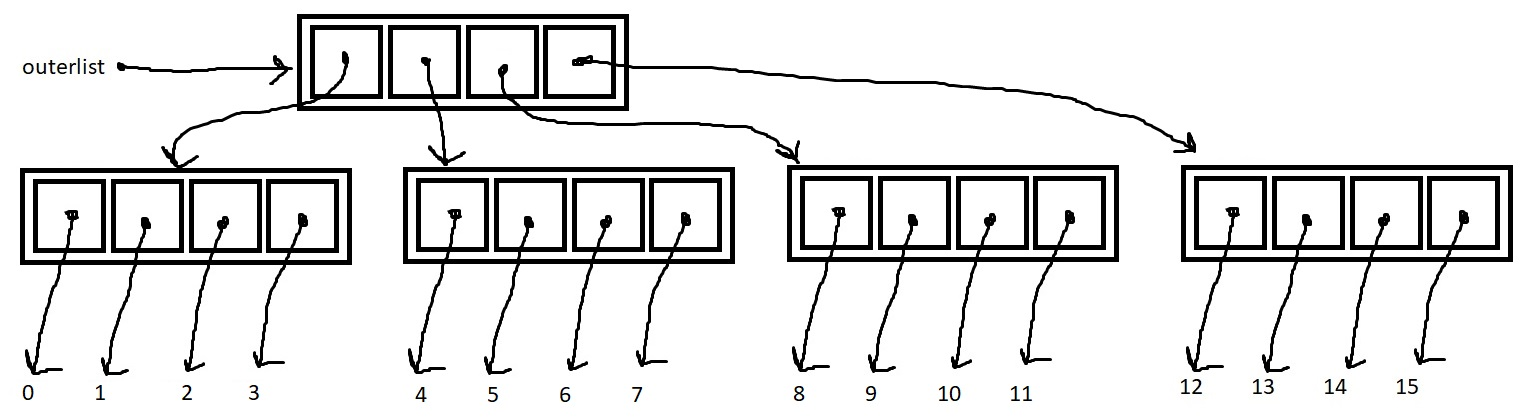
\includegraphics[width=\linewidth]{solution-incorrect-student-expectation.jpg}
\vspace{1em}

However, what we would find is that each element of the \texttt{outerList} just refers to the same \texttt{innerList}.

Following the links you would see all we are doing is overwriting the same list contents again and again, changing \texttt{innerList} from \texttt{[0,0,0,0]} to \texttt{[0,1,2,3]} to \texttt{[4,5,6,7]} to \texttt{[8,9,10,11]} to \texttt{[12,13,14,15]}.

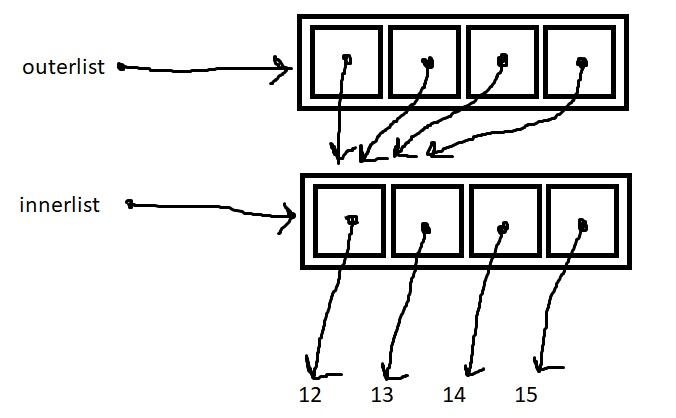
\includegraphics{solution-correct.jpg}\vspace{1em}

To implement this algorithm so that it matches expectations of a list of lists of 0 to 15, we need \textbf{different} inner lists, one for each cell.

\end{document}
